\chapter{Introduction} \label{chapter:introduction}
\section{Background}

Automatic Speech Recognition (ASR) systems, which convert human speech into text, have become integral to modern voice-driven technologies. While current commercial ASR solutions excel in single-language environments, they often struggle with multilingual scenarios, due to inter- and intra-sentence language variety \cite{code_switching}. The research team at Nanyang Technological University (NTU) Speech Lab addresses this challenge through their innovative multilingual ASR model, capable of transcribing speech in English, Malay, Mandarin, and Singlish \cite{speech_lab,scdf_2}. This development is particularly significant in Singapore's context, where code-switching between languages and dialects is commonplace in daily communication.

One prominent user of this ASR system is the Singapore Civil Defence Force (SCDF), which leverages the live transcription service for their emergency call centers \cite{scdf}. The transcription system enables officers to record key information efficiently, saving critical time during emergencies. Given the life-saving nature of these operations, the availability and reliability of the ASR system are paramount. Any system failure or disruption could severely hinder communication and delay emergency response efforts.

Currently, the ASR system is deployed on Kubernetes across Microsoft Azure and Amazon Web Services (AWS) cloud platforms. Figure \ref{fig:previous_architecture} illustrates the previous architecture of the ASR system. In this setup, users establish a WebSocket connection to the server, referred to as the Master Pod, via the NGINX Ingress Controller. The Master Pod then forwards audio data to a Worker Pod, which processes the transcription and returns the results to the user.

\begin{figure}[!ht]
    \centering
    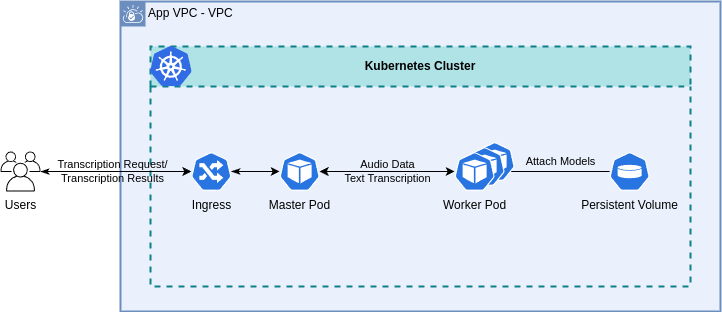
\includegraphics[width=\textwidth]{figures/previous_architecture.drawio.png}
    \caption{Previous Architecture of the ASR System}
    \label{fig:previous_architecture}
\end{figure}

\section{Challenges and Limitations}
Previous Final Year Project (FYP) students have contributed to various aspects of this ASR system, such as deploying it on AWS with Terraform \cite{song_yu, kai_shern} and enhancing its security \cite{putra}. However, several significant limitations persists:
\begin{enumerate}
    \item \textbf{Single Point of Failure:} The system relies on a single Master Pod, creating a single point of failure. If this pod crashes, there is no backup instance to handle requests, leading to potential service outages.
    \item \textbf{Tight Coupling:} The server and worker pods are tightly integrated, communicating synchronously via WebSocket connections. This restricts scalability, as components are highly dependent on each other, making it difficult to scale individual services independently \cite{tight_couple}.
    \item \textbf{Stateful Components:} Both the server and worker pods maintain state information, such as audio data and worker statuses. This reliance on stateful components complicates fault handling and exacerbates the system's lack of fault tolerance.
    \item \textbf{Worker Failures:} Worker pods can fail due to various reasons, including resource exhaustion, node crashes, or network disruptions. These failures leave audio processing tasks incomplete, disrupting the service. More importantly, worker failures directly impact the system’s ability to meet its Service Level Objectives (SLOs), particularly in terms of latency and availability.
    
\end{enumerate}

\section{Project Scope}
The objective of this FYP is to enhance the scalability and availability of the ASR system by transitioning to a decoupled architecture. The previous tightly coupled system struggles to handle fluctuating workloads and maintain service continuity during failures. To address these challenges, this project focuses on redesigning system components, improving scalability mechanisms, and enhancing failure recovery strategies.

\subsection{In Scope}
The project will address the following key areas:
\begin{enumerate}
    \item \textbf{Decoupling System Components with a Message Queue:} Introduce RabbitMQ as a message queue to facilitate asynchronous communication between the server and workers, enabling independent scaling and fault tolerance.
    \item \textbf{Developing a Dynamic and Predictive Scaling Policy for Workers:} Implement a dynamic scaling policy for worker pods that adjusts the number of instances based on real-time system load, ensuring optimal resource utilization and responsiveness.
    \item \textbf{Designing Mechanisms to Minimize Latency During Worker Failures:} Develop fault detection and recovery mechanisms to quickly identify and recover from worker failures, minimizing service disruptions and maintaining low latency.
\end{enumerate}

\subsection{Out-of-Scope}
While this project focuses on improving the system’s architecture and scalability, the following areas are beyond its scope:
\begin{itemize}
    \item \textbf{Modifications to the ASR Model:} The underlying speech recognition model used for transcription will remain unchanged. Enhancements to its accuracy, multilingual capabilities, or computational efficiency are beyond the project's focus.
    \item \textbf{Security Enhancements:} Although security is a critical aspect of any system, improvements such as encryption mechanisms, authentication, and access controls will not be covered in this research.
    \item \textbf{Monitoring and Observability:} While system performance will be evaluated, the project does not aim to build comprehensive logging, monitoring, or alerting frameworks beyond what is required for testing scalability and fault tolerance.
\end{itemize}

\section{Significance and Contributions}
This project significantly enhances the scalability, reliability, and fault tolerance of the ASR system, ensuring its availability under high-load conditions and unexpected failures. The improvements directly benefit NTU Speech Lab’s research initiatives and support critical applications such as SCDF’s emergency call centers, where real-time transcription is essential. 

By addressing the limitations of the existing architecture, this project makes the following key contributions:

\begin{itemize}
    \item \textbf{Decoupled System Architecture:} Introduced RabbitMQ as a message queue to enable asynchronous communication between system components, allowing independent scaling of workers and improving overall system robustness.
    
    \item \textbf{Dynamic and Predictive Worker Scaling:} Implemented an adaptive scaling policy for worker pods, dynamically adjusting the number of instances based on real-time system load to optimize resource utilization and responsiveness.

    \item \textbf{Automatic Scaling of Master Pods:} Configured autoscaling for Master Pods and other components based on CPU and memory consumption, ensuring efficient resource allocation.

    \item \textbf{Enhanced Fault Recovery Mechanisms:} Developed mechanisms for rapid detection and recovery of failed worker pods, reducing transcription disruptions and maintaining low-latency processing.

    \item \textbf{State Management with Redis:} Externalized application state management to Redis, reducing reliance on stateful components and improving resilience against crashes.

    \item \textbf{Deployment on Kubernetes with AWS:} Deployed the ASR system on Kubernetes clusters hosted on AWS, leveraging infrastructure-as-code tools like Terraform to streamline setup.

    \item \textbf{Refactored Codebase for Maintainability:} Restructured and modularized the existing codebase to align with the new architecture, enhancing maintainability, extensibility, and developer onboarding.

    \item \textbf{Comprehensive System Documentation:} Provided detailed documentation on system architecture, functionality, and key components to facilitate future development, troubleshooting, and maintenance.
\end{itemize}


\section{Report Organisation}
This report is structured into five chapters, each focusing on a specific aspect of the project:

\begin{itemize}
    \item \hyperref[chapter:introduction]{\textbf{Chapter 1: Introduction}} - This chapter provides an overview of the project, including its background, importance, objectives, scope, and significance.
    
    \item \hyperref[chapter:literature_review]{\textbf{Chapter 2: Literature Review}} - This chapter reviews previous FYP works on the ASR system and introduces the relevant technologies used in the project.
    
    \item \hyperref[chapter:analysis_and_design]{\textbf{Chapter 3: Analysis and Design}} - This chapter presents an analysis of the current ASR system architecture and identifies its limitations. It then describes the proposed decoupled architecture, including the use of message queues and dynamic scaling policies.
    
    \item \hyperref[chapter:detailed_implementation]{\textbf{Chapter 4: Detailed Implementation}} - This chapter provides a detailed implementation of the new architecture, the development of the dynamic scaling policy, and the mechanisms implemented to handle worker failures.
    
    \item \hyperref[chapter:conclusion_and_future_work]{\textbf{Chapter 5: Conclusion and Future Work}} - This chapter summarizes the contributions of the project. It also outlines potential areas for future research and development to further improve the ASR system.
\end{itemize}

